\documentclass[a4paper,12pt]{article} 

% packages and main settings
\usepackage[left=3cm, right=2cm, top=2cm, bottom=2cm]{geometry}
\usepackage[english]{babel}    
\usepackage[utf8]{inputenc}  
\usepackage[T1]{fontenc}        
\usepackage{lmodern}            
\usepackage{microtype}          
\usepackage{amsmath}
\usepackage{amsfonts, amsthm, amssymb, graphicx, booktabs}
\usepackage{bm} %bold epsilon
\usepackage{newclude}   
\usepackage{placeins}  %surpresses floating tables
\usepackage[labelfont=bf]{caption} %Figure etc steht dann in small caps 
\usepackage[labelsep=period]{caption} % dot after figure, table caption.
\usepackage[flushleft]{threeparttable} % for notes below table
\usepackage{multirow} % for table cell merge along rows
\usepackage{graphicx} % to adjust tablesize to textwidth
\usepackage{caption}  % for centered captions
\usepackage{float} % to set of autopositioning of tables
\usepackage[bottom,hang,flushmargin]{footmisc} % forces footnotes to the bottom
\usepackage{setspace}           % Fuer 1.5 fachen Zeilenabstand  
\onehalfspacing % 1.5 cm Zeilenabstand
%Bibtex
\usepackage[round,sort&compress]{natbib}

\bibliographystyle{chicago} % chicago bib style like in AER
\usepackage[hidelinks]{hyperref} % fuer links und verweise. Cleverref ist eigentlich besser. 


% Create header. The header must be surpressed for 
% every first page per section and a solution
% for the Appendix is used in the respective subfile.
\usepackage{fancyhdr}
\pagestyle{fancy}
\fancyhf{}
\chead{\nouppercase{\textit{\leftmark}}}
\cfoot{\thepage}
\renewcommand{\headrulewidth}{0pt} % no vertical line

%\usepackage{lipsum}  % check if formats work

\usepackage{afterpage} %clearpage w/o pagebreak for "header bug"

% Expectation symbol
\DeclareMathOperator*{\E}{\mathbb{E}}

% thin space, limits underneath in displays
% for strike through
\DeclareMathOperator*{\argmax}{argmax}
\newcommand*{\defeq}{\stackrel{\text{def}}{=}}
\usepackage[normalem]{ulem}
% try to use strikeout in section headers and others
\DeclareRobustCommand{\hsout}[1]{\texorpdfstring{\sout{#1}}{#1}}

% for gray table row color
\usepackage[table]{xcolor}

% decimal dot alignment in table columns
\usepackage{siunitx}

% for footnotes in table
\usepackage[flushleft]{threeparttable}

% for underbar
\newcommand{\ubar}[1]{\text{\b{$#1$}}}

\usepackage{tikz}

% Setup for urls
\usepackage{url}

\defcitealias{Respy-Stenzel.2019}{\textit{respy}}
\defcitealias{Gabler.2019}{\textit{estimagic}}
\defcitealias{Stenzel.2020}{\textit{Master's Thesis Replication Repository}}
\defcitealias{NLSY79}{NLSY79}


\usepackage{tikz}


\usepackage{enumitem}



\begin{document}

\newpage % delete after section is complete

\section{Qualitative GSA measures for functions with correlated input parameters}
\thispagestyle{plain} % suppress header on first page

This chapter explains the computation of the EE-based screening measures that are applied to the model in \cite{Keane.1994}.
First, I outline two sampling schemes that are tailored to the computation of EEs. Second, I present a simplified version of the approach to extend EEs to models with correlated parameters by \cite{ge2017extending}. Third, I develop an improvement to these measures that sustains the EE's fundamental derivative characteristic. The section concludes with the analysis of a test function. This analysis shows, first, my ability to replicate the results in \cite{ge2017extending}, and second, validates my improvement.


\subsection{Sampling Schemes}

The two presented sampling schemes are the trajectory and the radial design. Although the schemes are tailored to the computation of EEs, positional differences between them cause differences in their post-processing to compute the measures.\\

\noindent
According to several experiments with common test functions by \cite{campolongo2011screening}, the best design is the radial design (\cite{saltelli2002making}) and the most commonly used is the trajectory design (\cite{Morris.1991}).
Both designs are comprised by a $(k + 1) \times k$-dimensional matrix. The elements are generated in $[0,1]$. Afterwards, they can potentially be transformed to the distributions of choice. The columns represent the different input parameters and each row is a complete input parameter vector. To compute the aggregate qualitative measures, a set of multiple matrices, or sample subsets, of input parameters has to be generated.\\

\noindent
A matrix in radial design is generated the following way: Draw a vector of length $2k$ from a quasi-random sequence. The first row, or parameter vector, is the first half of the sequence. Then, copy the first row to the remaining $k$ rows. For each row $k'$ of the remaining 2, ..., $k+1$ rows, replace the $k'$-th element by the $k'$-th element of the second half of the vector. This generates a matrix of the following form:
\begin{align}
\underset{(k+1)\times k}{\bold{R}} =
\begin{pmatrix}
a_1 & a_2 & ... & a_k \\
\bold{b_1} & a_2 & ... & a_k \\
a_1 & \bold{b_2} & ... & a_k \\
\vdots & \vdots & 	\ddots & \vdots\\
a_1 & a_2 & ... & \bold{b_k}
\end{pmatrix}
\end{align}
\noindent
Note here, that each column consists only of the respective first row element, except of in one row.
From this matrix, one EE can be obtained for each parameter $X_i$. This is achieved by using the $(i+1)$-th row as function argument for the minuend and the first row as the subtrahend in the EE formula in Equation (\ref{eq:EE}). Then, $\Delta^{(i,j)} = b_i^{(j)} - a_i^{(j)}$. The asterisk is an index for all elements of a vector.
\begin{align} \label{eq:rad}
d_i =  \frac{Y(\bold{a_{\sim i}}, b_i) - Y(\bold{a})}{b_i - a_i} = \frac{Y(\bold{R_{i+1,*}}) -  Y(\bold{R_{1,*}})}{b_i - a_i}.
\end{align}
If the number of radial subsamples is high, the draws from the quasi-random sequence lead to a fast coverage of the input space (compared to a random sequence). However, a considerable share of steps will be large, at maximum $1-\epsilon$ in a sample space of $[0,1]$. This amplifies the aforementioned problem of EE-based measures with non-linear functions. The quasi-random sequence considered here is the Sobol' sequence. It is comparably successful in the dense coverage of the unit hypercube, but also conceptually more involved. Therefore, its presentation is beyond the scope of this work. As the first elements of each Sobol' sequence, the direction numbers, are equal, I draw the sequence at once for all sets of radial matrices.\\

\noindent
Next, I present the trajectory design. As we will see, it can lead to a relatively representative coverage for a very small number of subsamples but also to repetitions of similar draws.
I skip the equations that generate a trajectory and present the method verbally instead.
There are different forms of trajectories. I focus on the common version presented in \cite{Morris.1991} that generates equiprobable elements. The first step is to decide the number $p$ of equidistant grid points in interval $[0,1]$. Then, the first row of the trajectory is composed of the lower half value of these grid points. Now, fix $\Delta = p/[2(p-1)]$. This function implies, that adding $\Delta$ to the lowest point in the lowest half results in the lowest point of the upper half of the grid points, and so on. It also implies that 0.5 is the lower bound of $\Delta$. The rest of the rows is constructed, first, by copying the row one above and, second, by adding $\Delta$ to the $i$-th element of the $i+1$-th row. The created matrix scheme is depicted below.
\begin{align}
\underset{(k+1)\times k}{\bold{T}} =
\begin{pmatrix}
a_1 & a_2 & ... & a_k \\
\bold{b_1} & a_2 & ... & a_k \\
\bold{b_1} & \bold{b_2} & ... & a_k \\
\vdots & \vdots & 	\ddots & \vdots\\
\bold{b_1} & \bold{b_2} & ... & \bold{b_k}
\end{pmatrix}
\end{align}
\\

\noindent
In contrary to the radial scheme, each $b_i$ is copied to the subsequent row. Therefore, the EEs have to be determined by comparing each row with the row above instead of with the first row.
Importantly, two random transformations are common. These are, first, randomly switching rows, and second, randomly interchanging the $i$-th column with the $(k-i)$-th column and then reversing the column. The first transformation is skipped as it does not add additional coverage and because we need the stairs-shaped design to facilitate later transformations which account for correlations between input parameters. The second transformation is adapted because it is important to also have negative steps and because it sustains the stairs shape. Yet, this implies that $\Delta$ is also parameter- and trajectory-specific. Let $f$ and $h$ be additional indices representing the input parameters. The derivative formula is adapted to the trajectory design as follows:\footnote{In contrary to most authors, I also denote the step as a subtraction instead of $\Delta$ when referring to the trajectory design. This provides additional clarity.}

\begin{align} \label{eq:traj}
d_i =  \frac{Y(\bold{b_{f \leq i}}, \bold{a_{h>i}}) - Y(\bold{b_{f<i}}, \bold{a_{h \geq i}})}{b_i - a_i} = \frac{Y(\bold{T_{i+1,*})} -  Y(\bold{T_{i,*}})}{b_i - a_i}.
\end{align}
The trajectory design involves first, a fixed grid, and second and more importantly, a fixed step $\Delta$, s.t. $\{\Delta\} = \{\pm \Delta\}$. This implies less step variety and less space coverage vis-á-vis the radial design for larger number of draws.\\

\noindent
To improve the the sample space coverage by the trajectory design, \cite{campolongo2007effective} develop a post-selection approach based on distances. The approach creates enormous costs for more than a small number of trajectories. This problem is effectively mitigated by \cite{ge2014efficient}. The following describes the main ideas of both contributions.

The objective of both contributions is to select $k$ trajectories from a set of $N$ matrices. \cite{campolongo2007effective} assign a distance to each pair of trajectories in the start set. To each set of pair combinations in every possible subset of $k$ trajectories, \citeauthor{campolongo2007effective} assign an aggregate distance based on the pair distances. Then, the optimized trajectory set is the subset with the highest aggregate distance.

This is computationally very costly, because each aggregate distance is a sum of a binomial number of pair distances\footnote{For example, $\binom{30}{15} = 155117520$.}. To decrease the computation time, \cite{ge2014efficient} propose two improvements. First, in each iteration $i$, they select only $N(i)-1$ matrices from a set containing $N(i)$ trajectories until the set size has decreased to $k$. Second, they compute the pair distances in each iteration based on the aggregate distances and the pair distances from the first set. Due to numerical imprecisions, their improvement does not always result in the same set as obtained from \cite{campolongo2007effective}. However, the sets are usually very similar in terms of the aggregate distance. This thesis only uses the first step in \cite{ge2014efficient} to post-select the trajectory set because the second step does not provide any gain.\footnote{This refers only to my implementation.}\\


\noindent
So far, we have only considered draws in [0,1]. For uncorrelated input parameters from arbitrary distributions with well-defined CDF, $\Phi$, one would simply evaluate each element (potentially including the addition of the step) by the inverse CDF, or quantile function, $\Phi^{-1}$, of the respective parameter. One intuition is, that $\Phi$ maps the sample space to [0,1]. Hence $\Phi^{-1}$ can be used to transform random draws in [0,1] to the sample space of the arbitrary distribution. This is a basic example of so-called inverse transform sampling which we will recall in the next section.



\subsection{The approach for correlated input parameters in \cite{ge2017extending}}

This section describes the incomplete approach by \cite{ge2017extending} to extend the EE-based measures to input parameters that are correlated. Their main achievement is to outline a transformation of samples in radial and trajectory design that incorporates the correlation between the input parameters. This implies, that the trajectory and radial samples cannot be written as in Equation (\ref{eq:rad}) and Equation (\ref{eq:traj}). The reason is that the correlations of parameter $X_i$, to which step $\Delta^i$ is added, imply that all other parameters $\bold{X_{\sim i}}$ in the same row with non-zero correlation with $X_i$ are changed as well. Therefore, the rows cannot be denoted and compared as easily by $a$'s and $b$'s as in Equation (\ref{eq:rad}) and (\ref{eq:traj}). Transforming these matrices allows to re-define the EE-based measures accordingly, such that they sustain the main properties of the ordinary measures for uncorrelated parameters. The property is being a function of the mean derivative. Yet, \cite{ge2017extending} do not fully develop these measures. I explain how their measures lead to arbitrary results for correlated input parameters. This section covers their approach in a simplified form, focussing on normally distributed input parameters, and presents their measures.\\

\noindent
The next paragraph deals with developing a recipe for transforming draws $\bold{u} = \{u_1, u_2, ..., u_k\}$ from $[0,1]$ for an input parameter vector to draws $\bold{x} = \{x_1, x_2, ..., x_k\}$ from an arbitrary joint normal distribution. We will do this in three steps. 

For this purpose, let $\bold{\Sigma}$ be a non-singular variance-covariance matrix and let $\pmb{\mu}$ be the mean vector. The $k$-variate normal distribution is denoted by $\mathcal{N}_k(\pmb{\mu}, \bold{\Sigma})$. \\

\noindent
Creating potentially correlated draws $\bold{x}$ from $\mathcal{N}_k(\pmb{\mu}, \bold{\Sigma})$ is simple. Following \cite{gentle2006random}\footnote{See p. 197}, this can be achieved the following way: Draw a $k$-dimensional row vector of i.i.d standard normal deviates from the univariate $N(0,1)$ distribution, such that  $\bold{z} = \{z_1, z_2, ..., z_k\}$, and compute the Cholesky decomposition of $\Sigma$, such that $\bold{\Sigma} = \bold{T^T T}$. The lower triangular matrix is denoted by $\bold{T^T}$. Then apply the operation in Equation (10) to obtain the correlated deviates from $\mathcal{N}_k(\pmb{\mu}, \bold{\Sigma})$.
\begin{align}
\bold{x} = \pmb{\mu} + \bold{T^T z^T} 
\end{align}
Intuition for the underlying mechanics is provided in Appendix A. \\

\noindent
The next step is to understand that we can split the operation in Equation (10) into two subsequent operations. The separated first part allows to potentially map correlated standard normal deviates to other distributions than the normal one. For this, let $\pmb{\sigma}$ be the vector of standard deviations and let $\bold{R_k}$ be the correlation matrix of $\bold{x}$.

The first operation is to transform the standard deviates $\bold{z}$ to correlated standard deviates $\bold{z_c}$ by using $\bold{z_c}=\bold{Q^T z^T}$. In this equation, $\bold{Q^T}$ is the lower matrix from the Cholesky decomposition $\bold{R_k}=\bold{Q^T Q}$. This is equivalent to the above approach in \cite{gentle2006random} for the specific case of the multivariate standard normal distribution $\mathcal{N}_k(0, R_k)$. This is true because for multivariate standard normal deviates, the correlation matrix is equal to the covariance matrix.

The second operation is to scale the correlated standard normal deviates: $\bold{z}=\bold{z_c(i)}\pmb{\sigma}\bold{(i)} + \pmb{\mu}$., where the $i$s indicate an element-wise multiplication. This equation is specific to normally distributed parameters.\\

\noindent
The last step to construct the final approach is to recall the inverse transform sampling method. Therewith, we can transform the input parameter draws $\bold{u}$ to uncorrelated standard normal draws $\bold{z}$. Then we will continue with the two operations in the above paragraph. The transformation from $\bold{u}$ to $\bold{z}$ is denoted by $ F^{-1}(\Phi^c)$, where the $c$ in  $\Phi^c$ stands for the introduced correlations. This transformation is summarized by the following three steps:


\[
\left.\parbox{0.5\textwidth}{%
\begin{enumerate}[label=\bfseries Step \arabic*:,leftmargin=*,labelindent=5em]
	\item $\bold{z} = \pmb{\Phi^{-1}({u})}$
    \item $\bold{z_c} = \bold{Q^T z^T}$
    \item $\bold{x} = \pmb{\mu} + \bold{z_c(i)}\pmb{\sigma(i)}$
\end{enumerate}
}\right\}F^{-1}(\Phi^c) \defeq \mathcal{T}_2
\]

\noindent
To map $u$ to different sample spaces, Step 3 can be substituted. For instance, this could be achieved by applying $\Phi^u$, and the inverse CDF of the desired distribution to $z_c$.\footnote{The procedure described in the three steps above is equivalent to an inverse Rosenblatt transformation and a linear inverse Nataf transformation for parameters in normal sample space and connects to Gaussian copulas. For the first two transformations, see \cite{lemaire2013structural}, p 78 - 113. These concepts can be used to transform deviates in [0,1] to the sample space of arbitrary distributions by using the properties sketched above under varying assumptions.}\\

\noindent
The one most important point to understand is that the transformation comprised by the three steps is not unique for correlated input parameters. Rather, the transformation changes with the order of parameters in vector $\bold{u}$\footnote{This point is more obvious in the formal definition of the Rosenblatt transformation.}. This can be seen from the lower triangular matrix $\bold{Q^T}$. To prepare the next equation, let $\bold{R_k} = (\rho_{ij})_{ij=1}^k$ and sub-matrix $\bold{R_h} = (\rho_{ij})_{ij=1}^h$, $h \leq k$. Also let $\pmb{\rho_i^{*,j}} = (\rho_{1,j}, \rho_{2,j}, ..., \rho_{i-1,j})$ for $j \geq i$ with the following abbreviation $\pmb{\rho_i}\defeq\pmb{\rho_i^{*,i}}$. Following \cite{madar2015direct}, the lower matrix can be written as

\begin{align} \label{eq:corr}
\bold{Q^T} =
\begin{pmatrix}
\\ 1 & 0 & 0 & ... & 0
\\\rho_{1,2} & \sqrt{1-\rho_{1,2}^2} & 0 & ... & 0
\\ \rho_{1,3} & \frac{\rho_{2,3}-\rho_{1,2}\rho_{1,3}}{\sqrt{1-\rho_{1,2}^2}} & \sqrt{1-\pmb{\rho_{3}}\bold{R^{-1}_2}\pmb{\rho_{3}^T}} & ... & 0
\\\vdots & \vdots & \vdots & 	\ddots & \vdots
\\ \rho_{1,k} &\frac{\rho_{2,k}-\rho_{1,2}\rho_{1,k}}{\sqrt{1-\rho_{1,2}^2}} & \frac{\pmb{\rho_{3,k}}-\pmb{\rho_{3}^{*,k}}\bold{R^{-1}_2}\pmb{\rho_{3}^T}}{\sqrt{1-\pmb{\rho_{3}}\bold{R^{-1}_2}\pmb{\rho_{3}^T}}}  &
... & \sqrt{1-\pmb{\rho_{k}}\bold{R^{-1}_2}\pmb{\rho_{k}^T}}
\end{pmatrix}.
\end{align}
Equation (\ref{eq:corr}), together with Step 2, implies that the order of the uncorrelated standard normal deviates $\pmb{z}$ constitutes a hierarchy amongst the correlated deviates $\bold{z_c}$ in the following manner: The first parameter is not subject to any correlations, the second parameter is subject to the correlation with the first parameter, the third parameter is subject to the correlations with the parameters before, etc. Therefore, if parameters are correlated, typically $\bold{Q^T z^T} \neq \bold{Q^T (z')^T}$ and $F^{-1}(\Phi)(\bold{u}) \neq F^{-1}(\Phi)(\bold{u'})$, where $\bold{z'}$ and $\bold{u'}$ denote $\bold{z}$ and $\bold{u}$ in different orders.

Coming back to the EE-based measures for correlated inputs, \cite{ge2017extending} attempt to construct two variations of $d_i$. They name one EE the independent Elementary Effects, $d_i^{ind}$, and the other one the full Elementary Effects, $d_i^{full}$. For each of these two EEs, they derive the aggreate measures $\mu$, $\mu^*$ and $\sigma$. The difference between the two EEs is that $d^{ind}$ excludes and $d^{full}$ includes the effect of the correlations from adding step $\Delta^i$ to $X_i$ on the other parameters $\bold{X_{\sim i}}$. Knowing $d_i^{ind}$ is important because the correlations can decrease $d_i^{full}$ (close to 0). However, if the independent-EE-based measures are not close to zero, $X_i$ is still important. Additionally, fixing this parameter can potentially change $d_i^{full}$ for $\bold{X_{\sim i}}$.\\

\noindent 
For the trajectory design, the formula for the full Elementary Effect, is given by
\begin{align} \label{eq:d_full}
d_i^{full,T} = \frac{f\big(\mathcal{T}(\bold{T_{i+1,*}}; i-1)\big) - f\big(\mathcal{T}(\bold{T_{i,*}}; i)\big)}{\Delta}.
\end{align}
In Equation (12), $\mathcal{T}(\cdot; i) \defeq \mathcal{T}_3\bigg(\mathcal{T}_2\big(\mathcal{T}_1(\cdot; i)\big); i\bigg)$. $\mathcal{T}_1(\cdot; i)$ orders the parameters, or row elements, to establish the right correlation hierarchy. $\mathcal{T}_2$, or $F^{-1}(\Phi^c)$, correlates the draws in $[0,1]$ and transforms them to the sample space. $\mathcal{T}_3(\cdot; i)$ reverses the element order back to the start, to be able to apply the subtraction in the numerator of the EEs row-by-row. Index $i$ in $\mathcal{T}_1(\cdot; i)$ and $\mathcal{T}_3(\cdot; i)$ stands for the number of first row elements that is cut and moved to the back of the row in the same order. Applying $\mathcal{T}(\bold{T_{i+1,*}}; i-1)$ and $\mathcal{T}(\bold{T_{i+1,*}}; i)$ to all rows $i$ of trajectory $\bold{T}$ as in Equation (12) gives the following two transformed trajectories:

\begin{align} \label{eq:t1_min}
\mathcal{T}_1(\bold{T_{i+1,*}}; i-1)
=
\begin{pmatrix}
a_k & a_1 & ... & ... &  a_{k-1} \\
\bold{b_1} & a_2 & ... & ... &  a_k \\
\bold{b_2} & a_3 & ... & ... &  \bold{b_1} \\
\vdots & \vdots & \vdots & 	\ddots &  \vdots\\
\bold{b_k} & \bold{b_{1}} & ... & ... &  \bold{b_{k-1}}
\end{pmatrix}
\end{align}
\begin{align} \label{eq:t1_sub}
\mathcal{T}_1(\bold{T_{i,*}}; i-1)=
\begin{pmatrix}
a_1 & a_2 & ... & ... &  a_k \\
a_2 & ... & ... &  a_k & \bold{b_1} \\
a_3 & ... & ... &  \bold{b_1} & \bold{b_2} & \\
\vdots & \vdots & \vdots & 	\ddots &  \vdots\\
\bold{b_1} & \bold{b_{2}} & ... & ... &  \bold{b_{k}}
\end{pmatrix}
\end{align}
Two points can be seen from Equation (\ref{eq:t1_min}) and (\ref{eq:t1_sub}). First, $\mathcal{T}_1(\bold{T_{i+1,*}}; i-1)$ and $\mathcal{T}_1(\bold{T_{i,*}}; i)$, i.e. the $(i+1)$-th row in Eq. (\ref{eq:t1_min}) and the $(i)$-th row in Eq. (\ref{eq:t1_sub}), only differ in the $i$-th element. The difference is $b_i - a_i$. Thus, these two rows can be used to compute the EEs like in the uncorrelated case in Equation (\ref{eq:EE}). However, in this order, the parameters are in the wrong positions to be directly handed over to the function, as the $i$-th parameter is always in front. The second point is that in $\mathcal{T}_1(\bold{T_{i+1,*}}; i-1)$, $b_i$ is in front of the $i$-th row. This order prepares the establishing of the right correlation hierarchy by $\mathcal{T}_2$, such that the $\Delta$ in $a_i + \Delta$ is included to transform all other elements representing $X_{\sim i}$. Importantly, to perform $\mathcal{T}_2$, mean vector $\bold{x}$ and covariance matrix $\pmb{\Sigma}$ and its transformed representatives have always to be re-ordered according to each row. 
Then, $\mathcal{T}_3$ restores the original row order and $d_i^{full}$ can comfortably be computed by comparing function evaluations of row $i+1$ in $\mathcal{T}(\bold{T_{i+1,*}}; i-1)$ with function evaluations of row $i$ in $\mathcal{T}(\bold{T_{i,*}}; i-1)$. Now, the two transformed trajectories only differ in the $i$-th element in each row $i$. \\

\noindent
The formula for the independent Elementary Effect for the trajectory samples is given by
\begin{align} \label{eq:d_ind}
d_i^{ind, T} = \frac{f\big(\mathcal{T}(\bold{T_{i+1,*}}; i)\big) - f\big(\mathcal{T}(\bold{T_{i,*}}; i)\big)}{\Delta}.
\end{align}

\noindent
Note that $\mathcal{T}(\bold{T_{i+1,*}}; i)$ equals $\mathcal{T}(\bold{T_{i,*}}; i-1)$ which is the function argument in the subtrahend in Equation (\ref{eq:d_full}). Therefore this transformation can be skipped for the trajectory design and the transformed trajectory in Equation (\ref{eq:d_ind}) can be recycled. Here, the $X_i$ that takes the step in the denominator of the Elementary Effect is moved to the back such that the step does not affect the other input parameters $\bold{X_{\sim i}}$ through the correlations. The left trajectory is constructed such that for each row $i$, $a_i$ does take the step that $b_i$ took in the aforementioned minuend trajectory. The argument of the subtrahend in the denominator in $d_i^{ind}$ is given by the rows in

\begin{align}
\mathcal{T}_1(\bold{T_{i,*}}; i-1)=
\begin{pmatrix}
a_2 & a_3 & ... & ... &  a_1 \\
a_3 & ... & a_k &  \bold{b_1} & a_2 \\
a_4 & ... & \bold{b_1} &  \bold{b_2} & a_3 & \\
\vdots & \vdots & \vdots & 	\ddots &  \vdots\\
\bold{b_2} & \bold{b_{3}} & ... & ... &  \bold{b_{1}}
\end{pmatrix}
\end{align}

\noindent
The transformation for the samples in radial design work equally except that the minuend samples are composed of the first row copied to each row below because the steps in the radial design are always taken from the draws in the first row. To account for the correlation hierarchy and the transformation to the sample space performed by $\mathcal{T}_2$, it is important to also reorder the minuend trajectories. In fact, it is enough to compute one minuend trajectory if the order is regarded correctly. The forumalae of the Elementary Effects for the radial design are given by Equation (17) and (18).

\begin{align}
d_i^{full, R} = \frac{f\big(\mathcal{T}(\bold{R_{i+1,*}}; i-1)\big) - f\big(\mathcal{T}(\bold{R_{1,*}}; i)\big)}{b_i - a_i}.
\end{align}

\begin{align}
d_i^{ind, R} = \frac{f\big(\mathcal{T}(\bold{R_{i+1,*}}; i)\big) - f\big(\mathcal{T}(\bold{R_{1,*}}; i)\big)}{b_i - a_i}.
\end{align}

\noindent
The trajectory scheme requires $N(3k+1)$ and the radial scheme $N3k$ function evaluations to compute both EEs. The first row of the minuend and the last row of the subtrahend trajectories can be skipped. If one transformed trajectory contains information for two EEs, then all rows are used for the trajectory design. The radial scheme requires one row evaluation less because the subsamples that contain the repeated first rows include a pair of identical rows.\\

\noindent
In the next section, I present the shortcomings of the EEs by \cite{ge2017extending}. 
Furthermore, I develop improved measures that finally correspond to the actual EE definition for uncorrelated parameters.


\subsection{Drawbacks in \cite{ge2017extending} and Corrected Elementary Effects.}

The drawback in the EE definitions by \cite{ge2017extending} is that $\Delta$ is transformed multiple times in the numerator but not in the denominator. Therefore, these measures are not Elementary Effects in the sense of a derivative. The transformation in the numerator is performed by applying $F^{-1}(\Phi^c)$ to $u_i^j = a_i^j + \Delta^{(i,j)}$. The corrected and slightly renamed measures are the correlated and the uncorrelated Elementary Effects, $d_i^{c}$ and $d_i^{u}$. They are given below for arbitrary input distributions and for samples in trajectory and radial design. Let ${Q^T}_{k,*k-1}$ be the last row except of the last element of the lower triangular Cholesky matrix of the correlation matrix in the respective order of $\mathcal{T}_1(\bold{T_{i+1,*}}; i-1)$ and $\mathcal{T}_1(\bold{T_{i+1,*}}; i-1)$. Let ${Q^T}_{k,k}$ be the last element of the same matrix. Let $\Phi^u$ be the transformation from $[0,1]$ to standard normal space without regarding correlations in Step 3. Let $F^{-1}$ be the transformation that maps standard normal deviates to an arbitrary sample space like in Step 1. Index $*k-1$ represents all elements except of the last one of a vector of length $k$. Index $j$ is used to indicate an element-wise multiplication. Then

\begin{align}
d_i^{c,T} = \frac{f\big(\mathcal{T}(\bold{T_{i+1,*}}; i-1)\big) - f\big(\mathcal{T}(\bold{T_{i-1,*}}; i)\big)}{F^{-1}\big(\Phi^u(b_i)\big) - F^{-1}\big( \Phi^u(a_i)\big)}
\end{align}

\begin{align} \label{eq:u1}
d_i^{u, T} = \frac{f\big(\mathcal{T}(\bold{T_{i+1,*}}; i)\big) - f\big(\mathcal{T}(\bold{T_{i,*}}; i)\big)}{F^{-1}\big({Q^T}_{k,*k-1}(j)T_{i+1,*k-1}^T(j) + {Q^T}_{k,k} \Phi^u(b_i)\big) - F^{-1}\big({Q^T}_{k,*k-1}(j)T_{i,*k-1}^T(j)+{Q^T}_{k,k} \Phi^u(a_i)\big)}
\end{align}

\begin{align}
d_i^{c, R} = \frac{f\big(\mathcal{T}(\bold{R_{i+1,*}}; i-1)\big) - f\big(\mathcal{T}(\bold{R_{1,*}}; i-1)\big)}{F^{-1}\big( \Phi^u(b_i)\big) - F^{-1}\big( \Phi^u(a_i)\big)}
\end{align}

\begin{align} \label{eq:u2}
d_i^{u, R} = \frac{f\big(\mathcal{T}(\bold{R_{i+1,*}}; i)\big) - f\big(\mathcal{T}(\bold{R_{1,*}}; i)\big)}{F^{-1}\big({Q^T}_{k,*k-1}(j)R_{i+1,*k-1}^T(j) + {Q^T}_{k,k} \Phi^u(b_i)\big) - F^{-1}\big({Q^T}_{k,*k-1}(j)R_{i,*k-1}^T(j)+{Q^T}_{k,k} \Phi^u(a_i)\big)}.
\end{align}

\noindent
In Equation (\ref{eq:u1}) and (\ref{eq:u2}), ${Q^T}_{k,*k-1}(j)R_{i,*k-1}^T(j)$ refers to the transformed trajectory of the copied first rows, $\mathcal{T}(\bold{R_{i+1,*}}; i)$, as previously described.

The denominator of the correlated Elementary Effect, $d_i^{c}$, consists of $\Phi$ and $F^{-1}$. These functions account for the transformation from uniform to arbitrary sample space. In $d_i^{c}$, the denominator must not account for a correlating transformation of $a_i$ and $b_i$ because ${Q^T}_{1,*} = (1, 0, 0, ..., 0)$.  Therefore, $b_i$ and $a_i$ are multiplied by one in the correlation step, Step 2, of the standard normal deviates.

The last point is not true for the uncorrelated Elementary Effect $d_i^{c,*}$. One accounts for the correlation step by multiplying $\Phi^u(b_i)$ by ${Q^T}_{k,*k-1}(j)T_{i+1,*k-1}^T(j)/\Phi^u(b_i)+{Q^T}_{k,k}$. The respective operation is also done for $\Phi^u(a_i)$. One can also write the denominator equally but less explicitly for all four EEs as $\cal{T}$$ (b_i) - \cal{T}$$ (a_i)$\footnote{From an implementation perspective, this is also the simplest and most general way. It only requires to transfer the right elements from the final, transformed samples to the denominator.}. Not accounting for $Q_t$ like \cite{ge2017extending} leads to arbitrarily decreased independent Elementary Effects for input parameters with higher correlations. As $d_i^{full}$ and $d_i^{ind}$ are interpreted jointly, both measures are in fact useless.

For $X_1, ..., X_k \sim \mathcal{N}_k(\pmb{\mu}, \bold{\Sigma})$, the denominator of $d_i^{u,*}$ simplifies drastically to

\begin{align}
\begin{split}
 \big(\mu_i + \sigma_i\big({Q^T}_{k,*k-1}(j)T_{i+1,*k-1}^T(j) + {Q^T}_{k,k} \Phi^u(b_i)\big) \\-  \big(\mu_i + \sigma_i\big({Q^T}_{k,*k-1}(j)T_{i+1,*k-1}^T(j) + {Q^T}_{k,k} \Phi^u(a_i)\big)\\= \sigma_i{Q^T}_{k,k}\big(\Phi^u(b_i)-\Phi^u(a_i)\big).
 \end{split}
\end{align}

\noindent
The next section presents results for a test function to demonstrate a replication of \cite{ge2017extending} and to validate this thesis' measures.

\subsection{Replication and Validation}

Let $f(X_1, ..., X_k)$ = $\sum_{i = 1}^{k} c_i X_i$ be an arbitrary linear function. Let $\rho_{i,j}$ be the linear correlation between $X_i$ and $X_j$. Then, for all $i \in 1, ..., k$,
\begin{align}
d_i^{u,*} = c_i \label{eq:diu}\\
d_i^{c,*} = \sum_{j = 1}^{k} \rho_{i,j} c_{j}. \label{eq:dic}
\end{align}
Both equations state that, conceptually, the result does not depend on the sampling scheme.

Equation (\ref{eq:diu}) shows that the uncorrelated EE of each input equals the derivative of $f(\bold{X})$ with respect to $X_i$. This corresponds to the concept of the original EE as a derivative. As the function is linear, the derivative is equal for all values in the sample space of each $X_i$. This implies $\mu=0$, $\mu^*=0 $ and $ \sigma=0$.

Equation (\ref{eq:dic}) states that the correlated EE of input parameter $X_i$ also includes the effects of the other input parameters that are correlated with $X_i$. As the model is linear, these effects are included by adding the respective coefficients multiplied by the correlation with $X_i$ to the uncorrelated effect, $d_i^{u,*}$.\footnote{These results correspond to the intuition provided by the example in \cite{Saltelli.2008}, page 123.}\\

\noindent
Table \ref{tab:repval1} and Table \ref{tab:repval2} show results for a simple linear test function with 3 input parameters, where $X_i \sim \mathcal{N}(0, 1)$ for $i=\{1,2,3\}$, and with correlations $\rho_{1,2}=0.9$, $\rho_{1,3}=0.4$, $\rho_{2,3}=0.01$. The first columns in both tables show the aggregate EE-based measures by \cite{ge2017extending}. The second (and third) columns show my replications for these measures. Table \ref{tab:repval1} consists of two replications because the trajectory design implies two numerical decisions. The details are explained in the following. The last columns in both tables depict the results for the measures developed in this thesis.
\newpage
% Please add the following required packages to your document preamble:
% \usepackage{booktabs}
\setlength{\tabcolsep}{12pt} %from 6
\begin{table}[H]
	\centering
	\caption{Replication and validation - trajectory design}
	\label{tab:repval1}
		\renewcommand{\arraystretch}{1.2}%
		\begin{threeparttable}
	\begin{tabular}{cS[table-format=3.2]S[table-format=3.2]S[table-format=3.2]S[table-format=3.2]}
		\toprule
		{Measure}     & {GM'17}   & {Repl. $\mu^{*}$}\tnote{$\dagger$} & {Repl. $\sigma$}\tnote{$\ddagger$} & {S'20} \\ \midrule


		& 1.20  & 1.36         & 0.83         & 1.00 \\
		\qquad $\mu^{*,ind}$                               & 1.30  & 1.48         & 0.91         & 1.00 \\
		& 3.20  & 3.11         & 1.94         & 1.00 \\
						&&&& \\
		& 0.55  & 0.00         & 0.56         & 0.00 \\
		\qquad $\sigma^{ind}$                            & 0.60  & 0.00         & 0.62         & 0.00 \\
		& 1.30  & 0.00         & 1.32         & 0.00 \\
						&&&& \\
		& 14.90 & 16.20        & 9.97         & 2.30 \\
		\qquad $\mu^{*,full}$                              & 12.50 & 13.45        & 8.31         & 1.91 \\
		& 10.00 & 9.93         & 6.18         & 1.41 \\
						&&&& \\
		& 6.50  & 0.00         & 6.74         & 0.00 \\
		\qquad $\sigma^{full}$                           & 5.50  & 0.00         & 5.63         & 0.00 \\
		& 4.00  & 0.00         & 4.20         & 0.00 \\		
\bottomrule	
\end{tabular}
  \begin{tablenotes}

	\item[$\dagger$] \footnotesize $0^{num}=0.00001$ and $l=4$. 
    \item[$\ddagger$] $0^{num}=0.00000001$ and $l=24$.\par

\end{tablenotes}
\end{threeparttable}
\end{table}

\hspace{1cm} %linebreak.
% Please add the following required packages to your document preamble:
% \usepackage{booktabs}
\setlength{\tabcolsep}{12pt} %from 6
\begin{table}[H]
	\centering
	\caption{Replication and validation - radial design}
	\label{tab:repval2}
	\renewcommand{\arraystretch}{1.2}%
	\begin{tabular}{cS[table-format=3.2]S[table-format=3.2]S[table-format=3.2]}
		\toprule
		{Measure}     & {GM'17}   & {Replication}  & {S'20} \\ 
		\midrule
		
		& 0.60  & 0.57         &  1.00 \\
		\qquad $\mu^{*,ind}$                               & 0.75  & 0.85         &  1.00 \\
		& 1.50  & 1.31         &  1.00 \\
		&&& \\
		& 0.20   & 0.10         &  0.00 \\
		\qquad $\sigma^{ind}$                            & 0.30   & 0.41         &  0.00 \\
		& 0.85  & 0.22         & 0.00 \\
		&&& \\
		& 7.50  & 6.84         &  2.30 \\
		\qquad $\mu^{*,full}$                              & 6.80   & 7.77         &  1.91 \\
		& 4.75  & 4.19         &  1.41 \\
		&&& \\
		& 2.90  & 1.15         &  0.00 \\
		\qquad $\sigma^{full}$                           & 2.65  & 3.68         &  0.00 \\
		& 2.50   & 0.70         &  0.00 \\ \bottomrule
	\end{tabular}
\end{table}

\newpage
\noindent
We can observe three things for the measures in \cite{ge2017extending} in the first columns. First the measures do not represent the derivative of $F$ with respect to $X_i$, as the non-linear transformation $F(\Phi^c(\cdot))$ is only applied to the EE numerator. This causes the second and third observations. The second one is that the measures differ between trajectory and radial design. This is because the non-linearity introduces variation to the measures. This reveals differences in sampling of the base values and the steps between the sampling schemes. Additionally, not enough samples have been drawn relative to the degree of variation. Therefore, the measures are noisy. Another reason for the differences between the measures based on radial and trajectory design in \cite{ge2017extending} are the two numerical parameters required by the trajectory design. These are. first, the approximation of $0$ and $1$ to prevent infinite values returned by the inverse CDF. It is enough to approximate $0$ by $0^{num}$. The lower $0^{num}$, the more extreme are the transformed draws for $0$ and $1$ The second approximation is the number of levels $l$, or grid points, in $[0,1]$. The more grid points, the less imprecise are the results.
The authors indicate that they use $0^{num}=0.00001$ and $l$ for the trajectory design.\footnote{I obtained this information from an unofficial email from Qiao Ge.} Additionally, the authors generated 240 trajectories and 260 radial samples. My figures base on 10,000 samples each. I replicate their measure for these parameters in the second column in Table \ref{tab:repval1}. The mean and mean absolute EEs, $\mu^{*,ind}$ and $\mu^{*,full}$ come reasonably close. However, the standard deviations, $\sigma^{*,ind}$ and $\sigma^{*,full}$ equal 0. The reason is that four grid points re-linearise the transformed numerator in the EEs. This argument is illustrated by Figure \ref{fig:invcdf}.



\begin{figure}[H]
	\caption{Grid points in standard normal sample space for trajectory design with $l=4$}
	\centering
	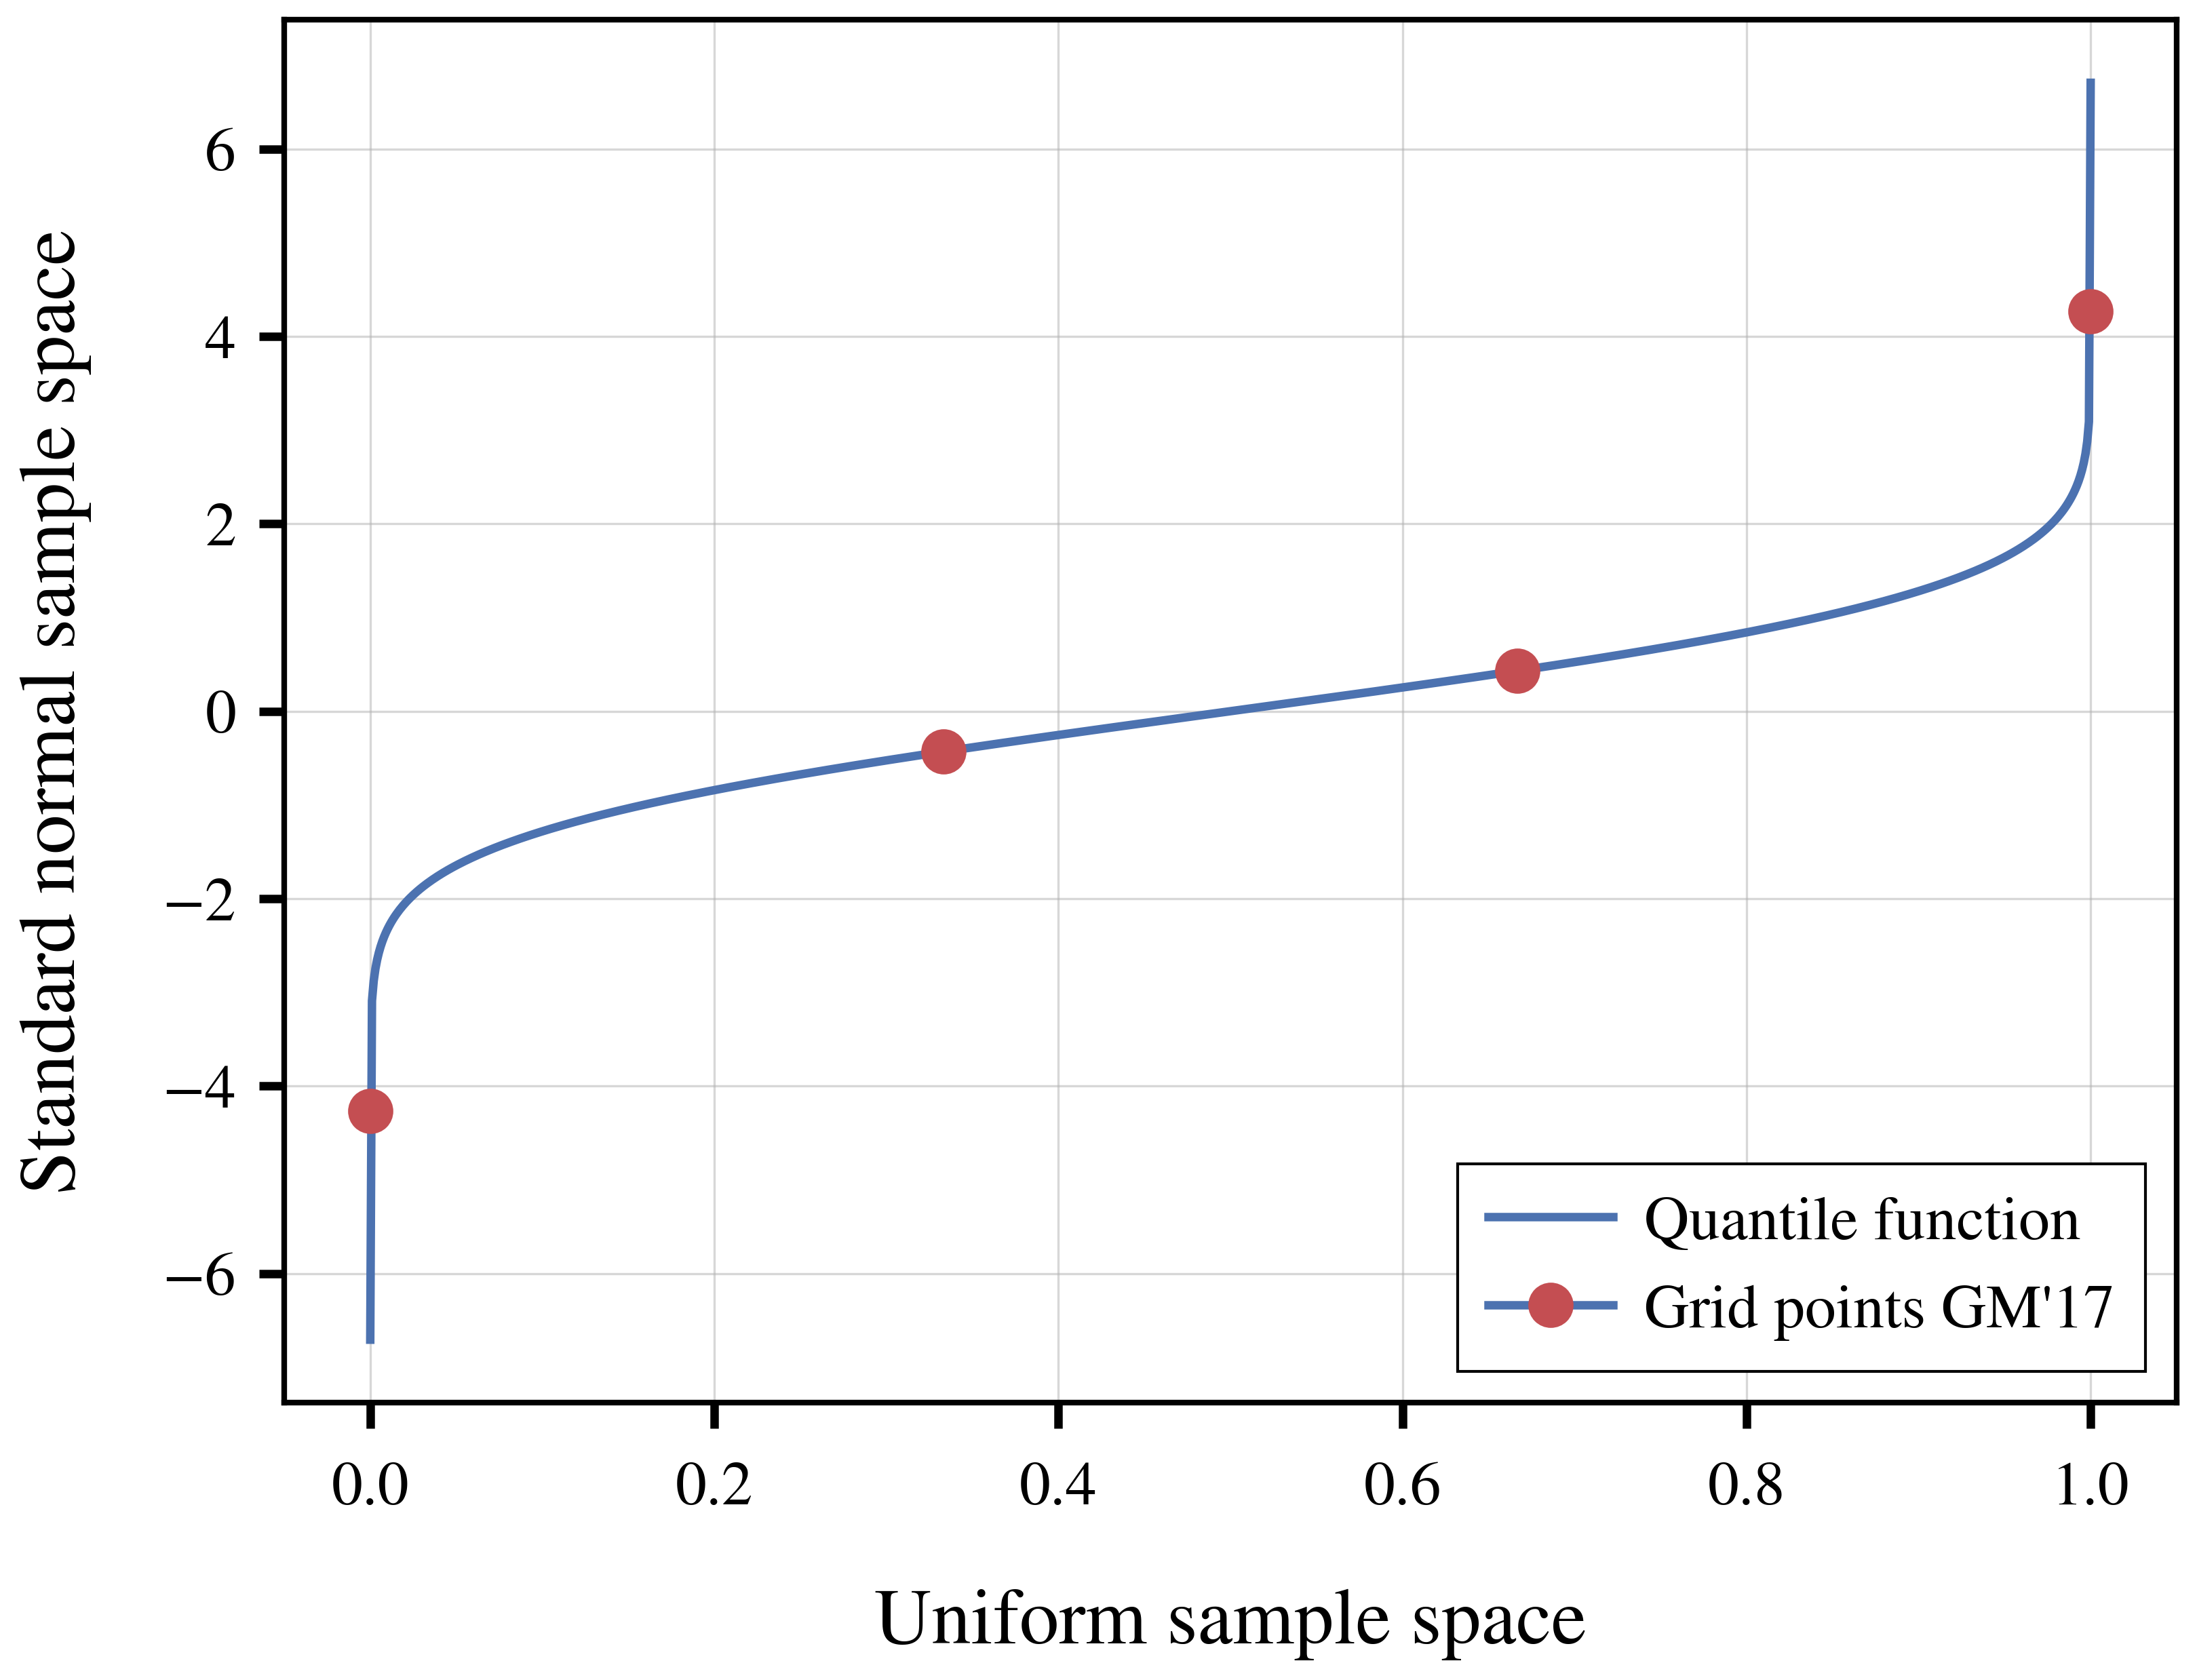
\includegraphics[scale=0.40]{../../../scrypy/figures/quantile_fct}
	\label{fig:invcdf}
\end{figure}

\noindent
The grid points with four levels are $ \{ 0^{num}, 1/3, 2/3, 1-0^{num} \}$ and $\Delta=2/3$. The quantile function is non-linear but point-symmetric to $(0.5, 0)$. Thus, $\Phi(\frac{1/3 - (1-0^{num})}{2/3}) = \Phi(\frac{0^{num} - 2/3}{2/3})$. Hence, the Elementary Effects are equal for each single $X_i$ because the transformed $\Delta$-specific derivation is equal at each of the two lower half grid points.\\

\noindent
Therefore, I used $0^{num}=0.00000001$ and $l=24$ to increase the variation amongst the EEs by \cite{ge2017extending} in order to achieve similar results.

The replication in Table \ref{tab:repval2} for the radial design is relatively close for the mean Effects. However, there are some differences for the standard deviations. In my opinion this results, first, from different start values from which the Sobol' sequence is generated, and second, from a too low number of samples in \cite{ge2017extending}. This indicates that the appropriate number of samples for correlated parameters has to be higher than what is common for functions with uncorrelated input parameters.

The last column in both Table \ref{tab:repval1} and Table \ref{tab:repval2} depicts the aggregate measures based on the improved EEs. These are equal to what is anticipated at the start of this section. Therefore, the correlated and uncorrealted Elementary Effects developed in this thesis can be regarded as a valid extension of Elementary Effects for models with correlated input parameters.\\

\noindent
The next chapter presents the occupational choice model in \cite{Keane.1994}.

\newpage
\bibliography{../../bibliography/literature}

\end{document}